% TEXINPUTS=.:$HOME/git/bvtex: latexmk  -pdf <main>.tex
\documentclass[xcolor=dvipsnames]{beamer}

\input{defaults}
\input{beamer/preamble}

\setbeamertemplate{navigation symbols}{}
% \setbeamertemplate{background}[grid][step=1cm]

\usepackage{forloop}
\usepackage{calc}
\usepackage{siunitx}
\usepackage{xmpmulti}
\usepackage[export]{adjustbox}
\usepackage{ulem}
\usepackage[outline]{contour}
\usepackage{tikz}
\usetikzlibrary{shapes.geometric, arrows}
\usetikzlibrary{positioning}

\definecolor{bvtitlecolor}{rgb}{0.98, 0.92, 0.84}
\definecolor{bvoutline}{rgb}{0.1, 0.1, 0.1}
\newcommand{\microboone}{MicroBooNE\xspace}
\renewcommand{\bvtitleauthor}{Brett Viren}
\renewcommand{\bvtit}{LARF}
\renewcommand{\bvtitle}{\LARGE 3D Field Inputs to Simulation}
\renewcommand{\bvevent}{BNL/\microboone\\21 Sep 2016}
\renewcommand{\bvbeamerbackground}{}



\def\Put(#1,#2)#3{\leavevmode\makebox(0,0){\put(#1,#2){#3}}}


\begin{document}
\input{beamer/title.tex}
\input{beamer/toc.tex}


\section{Impact Positions}
\subsection{0D}

\begin{frame}
  \frametitle{LArSoft Currently}

  \begin{itemize}
  \item 2D fields used to calculate response.
  \item Simulation induces signals only on nearest wire.
  \item A per-plane average response function used, no variation at
    sub-mm scale.
  \item Same average response function used for deconvolution.
    \begin{itemize}
    \item[$\Rightarrow$] absent noise, perfect deconvolution.
    \end{itemize}
  \end{itemize}
  Call this ``$\O$D'' (zero dimension) response simulation.

\end{frame}

\subsection{1D}

\begin{frame}[fragile]
  \frametitle{1D ``Impact Line''}
  \begin{center}
    Improved simulation (Xiaoyue)    
  \end{center}
  \begin{columns}
    \begin{column}{0.55\textwidth}
      \begin{itemize}\footnotesize
      \item $N_{paths}$ = 6 ``\textbf{impact positions}''
        \begin{itemize}\scriptsize
        \item one-side of U4 wire, 
        \item 1/10$^{th}$ pitch separation
        \end{itemize}
      \item $N_{wires}$ = 7 wires of interest
        \begin{itemize}\scriptsize
        \item weighting field for each wire
        \end{itemize}
      \item Exploit symmetries:
        \begin{itemize}\scriptsize
        \item Mirror about U4.
        \item Translation to reuse weighting field.
        \item Reciprocity to reuse impact positions.
        \end{itemize}
      \end{itemize}
    \end{column}
    \begin{column}{0.45\textwidth}
    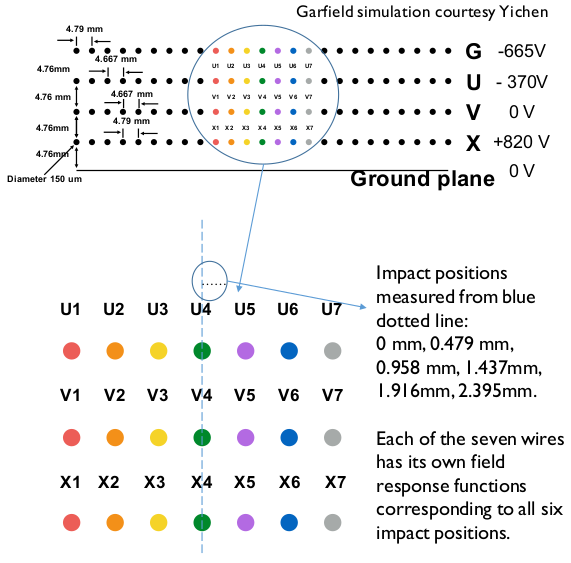
\includegraphics[width=0.95\textwidth,clip,trim=10mm 0 5mm 0]{xiaoyue-impact-positions.png}
    \end{column}
  \end{columns}
\end{frame}

\subsection{2D}

\begin{frame}
  \frametitle{Extension to 2D ``Impact Region''}
  Goals:
  \begin{itemize}
  \item Want to include the effects of 3D wire crossing pattern.
    \begin{itemize}\footnotesize
    \item Eventually handle complex DUNE crossings.
    \end{itemize}
  \item Retain exploitation of symmetries to minimize amount of computation.
    \begin{itemize}
    \item 2D necessarily requires more and produces larger result data.
    \end{itemize}
  \item Must organize response functions in a way to allow easy/fast
    lookup during simulation.
  \end{itemize}

  \begin{center}
    So, how to do this?
  \end{center}
\end{frame}

\usebackgroundtemplate{\includegraphics[width=\paperwidth,height=\paperheight]{ub-wire-lines.pdf}}
\begin{frame}
  \begin{center}
    $\mu$Boone wire crossing pattern
  \end{center}
  \vspace{6cm}
  \begin{center}
    What is the equivalent to the ``impact line'' here? 
  \end{center}
\end{frame}
\usebackgroundtemplate{}

\begin{frame}
  \frametitle{Minimum Unique 2D Region}

  \begin{columns}
    \begin{column}{0.5\textwidth}
      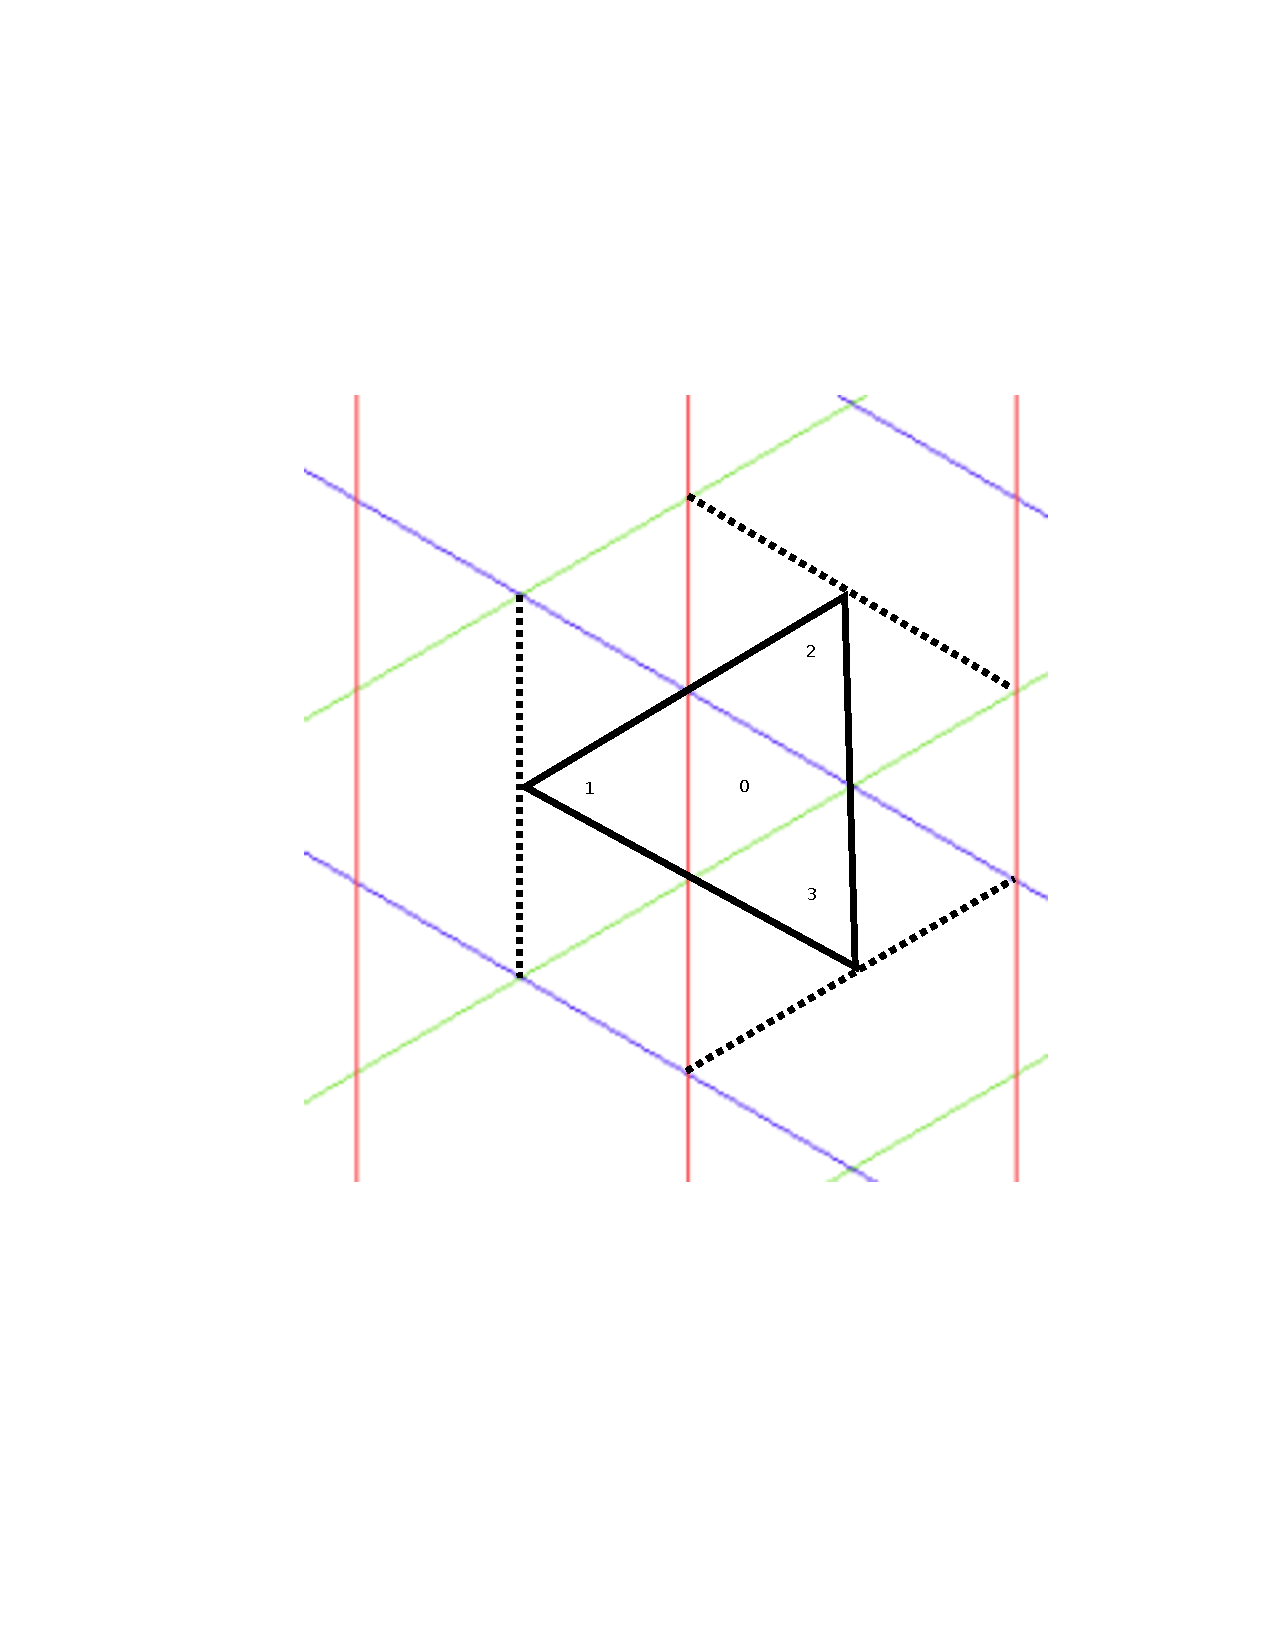
\includegraphics[width=\textwidth,clip,trim=4cm 6cm 4cm 6cm]{impact-triangle.pdf}      
    \end{column}

    \begin{column}{0.5\textwidth}
      Can map any point on the plane into black triangle while
        preserving the distance to the closest U/V/W wires.
        \begin{itemize}\scriptsize
        \item DUNE will require a more complex polygon of about 6 wires in size.
        \end{itemize}
      
        This particular ``impact triangle'' is just one of many
        possible choices.
    \end{column}

  \end{columns}

\end{frame}

\begin{frame}
  \frametitle{2D Impact Positions}
  
  \begin{center}
    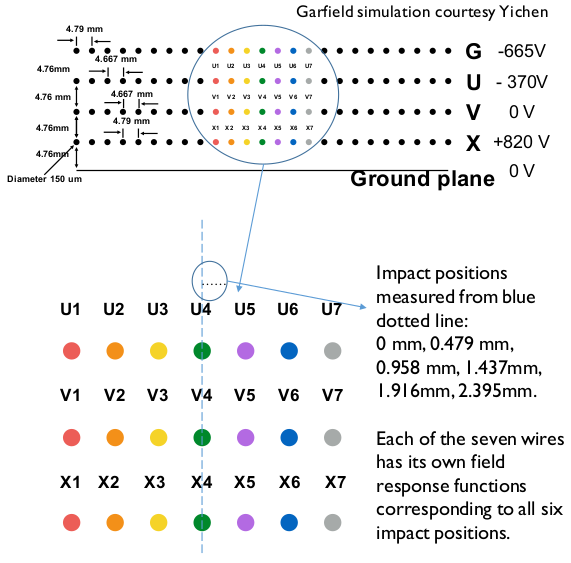
\includegraphics[width=0.5\textwidth,clip,trim=5cm 5cm 0cm 8cm]{xiaoyue-impact-positions.png}    

    \vfill

    What are the ``right'' 2D-equivalent impact positions?
  \end{center}
  

\end{frame}

\newcounter{bifurcateno}

\begin{frame}[fragile]
  \frametitle{Binning the Impact Triangle}

  \begin{columns}
    \begin{column}{0.6\textwidth}
      \forloop{bifurcateno}{1}{\value{bifurcateno}<8}{
        \only<\value{bifurcateno}>{%
          \includegraphics[height=5.5cm,page=\value{bifurcateno},clip,trim=0 1cm 0 1cm]{test_triangles_class.pdf} 
        }

      }

    \end{column}
    \begin{column}{0.4\textwidth}
      \only<1>{%
        \begin{description}
        \item[$N_{split}$] 0
        \item[$N_{pos}$] 3
        \item[$N_{\bigtriangleup}$] 1
        \item[res] 3.5mm
        \end{description}}
      \only<2>{%
        \begin{description}
        \item[$N_{split}$] 1
        \item[$N_{pos}$] 6
        \item[$N_{\bigtriangleup}$] 4
        \item[res] 1.7mm
        \end{description}}
      \only<3>{%
        \begin{description}
        \item[$N_{split}$] 2
        \item[$N_{pos}$] 15
        \item[$N_{\bigtriangleup}$] 16
        \item[res] 0.87mm
        \end{description}}
      \only<4>{%
        \begin{description}
        \item[$N_{split}$] 3
        \item[$N_{pos}$] 45
        \item[$N_{\bigtriangleup}$] 64
        \item[res] 0.43mm
        \end{description}}
      \only<5>{%
        \begin{description}
        \item[$N_{split}$] 4
        \item[$N_{pos}$] 153
        \item[$N_{\bigtriangleup}$] 256
        \item[res] 0.22mm
        \end{description}}
      \only<6>{%
        \begin{description}
        \item[$N_{split}$] 5
        \item[$N_{pos}$] 561
        \item[$N_{\bigtriangleup}$] 1024
        \item[res] 0.11mm
        \end{description}}
      \only<7>{%
        \begin{description}
        \item[$N_{split}$] 6
        \item[$N_{pos}$] 2145
        \item[$N_{\bigtriangleup}$] 4096
        \item[res] 0.05mm
        \end{description}}
    \end{column}
  \end{columns}
  \begin{itemize}\scriptsize
  \item Start with fundamental triangle.
  \item Recursively bifurcate sides until reaching approximate
    desired resolution.
  \item Color is arbitrary (sum of point indices).
  \end{itemize}

\end{frame}

\begin{frame}
  \frametitle{Bin Indexing}

  Given point in plane, how to find triangular bin, \textbf{quickly}?

  \vfill

  \begin{itemize}
  \item Can recursively check if point is inside triangle, then daughters.
    \begin{itemize}\footnotesize
    \item[$\rightarrow$] Simple and implemented in LARF but $\mathcal{O}(N_{split})$.
    \end{itemize}
  \item Can directly index based on distance from point to nearest
    wire in each plane.
    \begin{itemize}\footnotesize
    \item[$\rightarrow$] I still need to think how to do it but $\mathcal{O}(1)$.
    \end{itemize}
  \item In any case, this is needed on C++ side, not LARF.
  \end{itemize}

  \vfill

  Neither optimization method will extend exactly to the DUNE case.
\end{frame}

\begin{frame}
  \frametitle{Preparation of Inputs for Simulation}
  \setbeamercovered{transparent}
  \begin{columns}
    \begin{column}{0.5\textwidth}
      \begin{itemize}[<+->]\footnotesize
      \item<1> Define region of impact positions, in practice, sample
        a larger region and form average to reduce BEM artifacts.
      \item<2> Step through drift field for each start point to make path.
      \item<3> For each drift path, sample $3N_{wires} = 30$ weighting fields.
        Really, reuse 3 boundary condition solutions, as can offset drift paths by $n\times pitch$.
      \end{itemize}
    \end{column}
    \begin{column}{0.5\textwidth}
      \only<1>{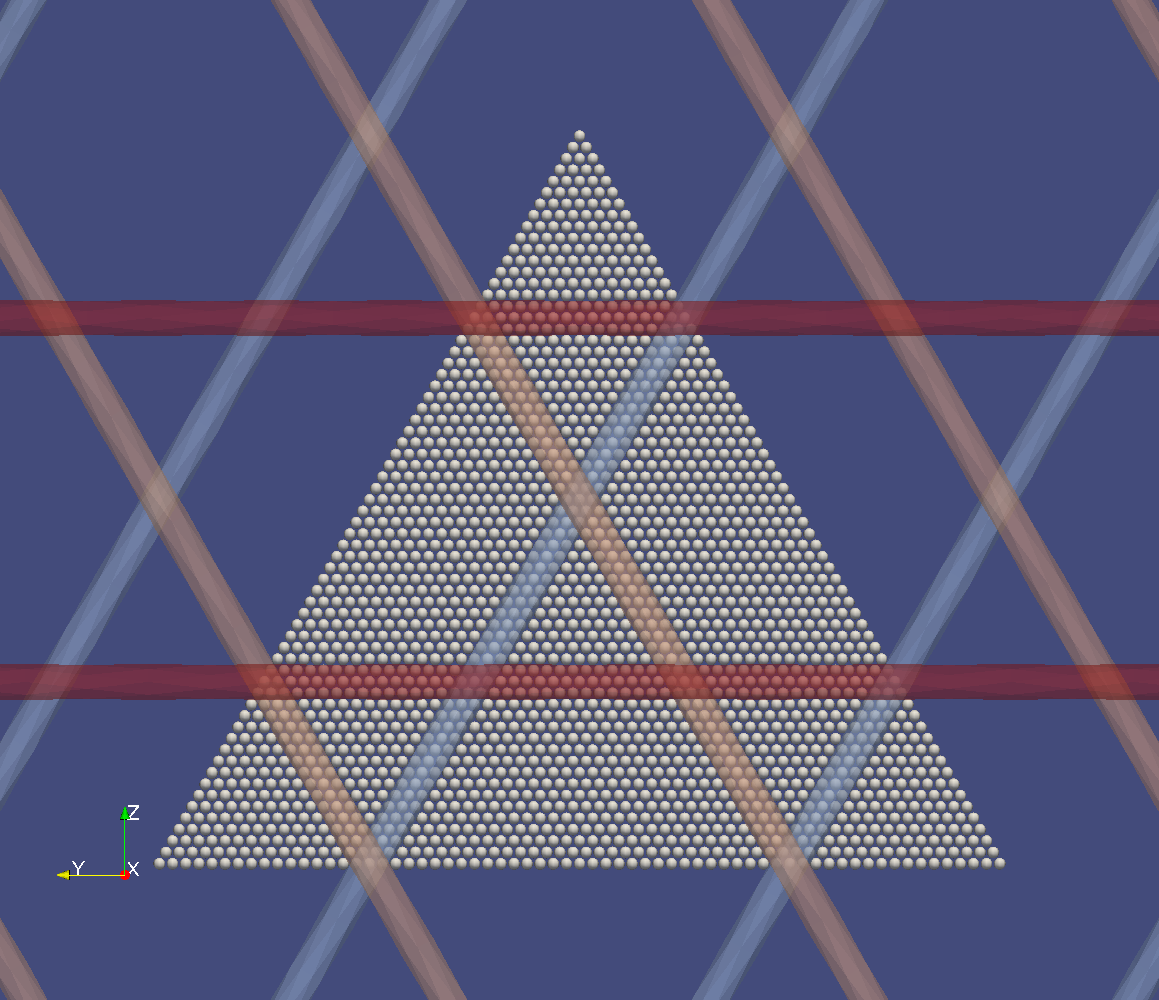
\includegraphics[width=\textwidth]{triangle-path-starts.png}}
      \only<2>{
        \begin{center}
          Processing now.\\
          (runs at about 1mm/hour,\\
          need to step 20mm....)
        \end{center}}
      \only<3>{
        \begin{center}
          (t.b.d.)
        \end{center}}
    \end{column}
  \end{columns}

\end{frame}

\section{Integration with Simulation}

\begin{frame}
  \frametitle{Integration with Simulation}
  LARF will provide $N_{pos} \times N_{plane} \times N_{wire}$ response functions.
  \begin{itemize}
  \item Match Xiaoyue: $N_{split} = 3 \to N_{pos} = 45, res = 0.43$ mm
    \begin{itemize}\footnotesize
    \item Currently generating $N_{split} = 6 \to N_{pos} = 2145, res = 0.05$ mm
    \end{itemize}
  \item Evaluate responses for $N_{plane} = 3, N_{wire} = 10$.
  \end{itemize}

  \vfill

  New C++ dev on simulation side:
  \begin{itemize}
  \item Select interchange file format to hold response data and
    develop some code to read it in.
    \begin{itemize}\footnotesize
    \item Probably JSON since this is easy and JSONCPP is already a dep.
    \end{itemize}
  \item Implement fast index/look-up of a response function given an
    arbitrary $\vec{r}$ projected to the path start plane (x=20mm).
  \end{itemize}

  \vfill

  Do this C++ work inside Wire Cell Toolkit?

\end{frame}

\end{document}

%%% Local Variables:
%%% mode: latex
%%% TeX-master: t
%%% End:
